\documentclass[3pt,landscape]{article}

\usepackage[utf8]{inputenc}
\usepackage{multicol}
\usepackage{parskip}
\usepackage{tabularx}
\usepackage{amsmath}
\usepackage{amssymb}
\usepackage{amsthm}
\usepackage{geometry}
\usepackage{booktabs}
\usepackage{centernot}
\usepackage{hyperref}
\usepackage{eufrak}
\usepackage{graphicx}
\graphicspath{{pics/}}
\geometry{a4paper, left=3mm, right=3mm, top=3mm, bottom=3mm}

\pagenumbering{gobble}

\begin{document}

\raggedright{}
\begin{multicols}{3}
    07.02
    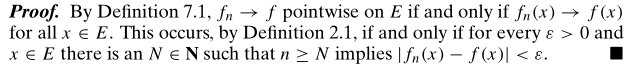
\includegraphics[width=250]{07_02.png} \\
    07.03a
    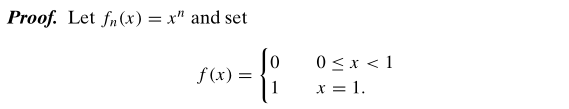
\includegraphics[width=250]{07_03a.png} \\
    07.03b
    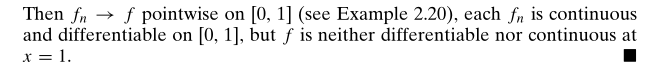
\includegraphics[width=250]{07_03b.png} \\
    07.04
    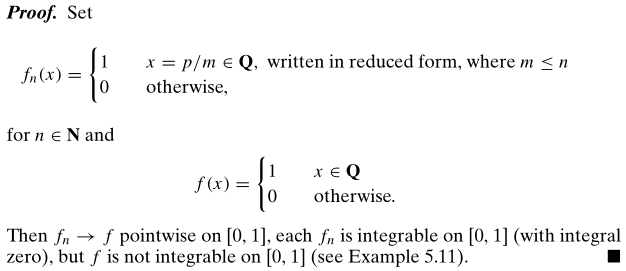
\includegraphics[width=250]{07_04.png} \\
    07.05
    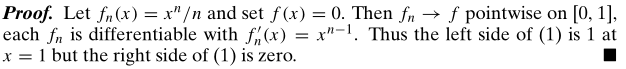
\includegraphics[width=250]{07_05.png} \\
    07.06
    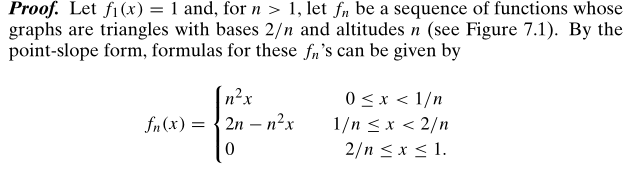
\includegraphics[width=250]{07_06a.png} \\
    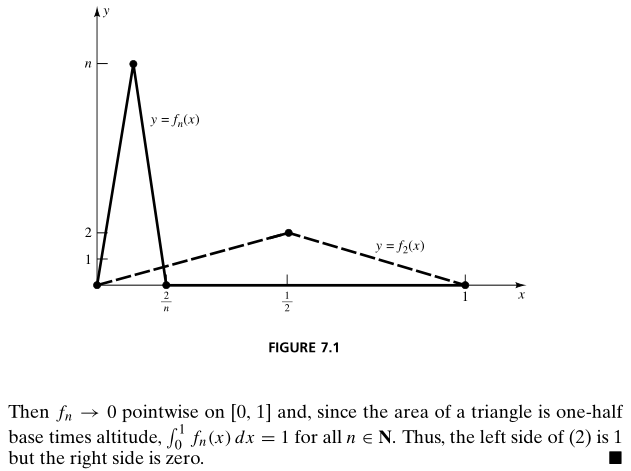
\includegraphics[width=250]{07_06b.png} \\
    07.09
    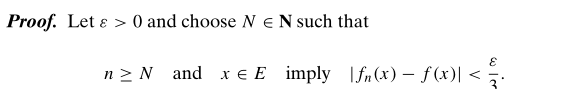
\includegraphics[width=250]{07_09a.png} \\
    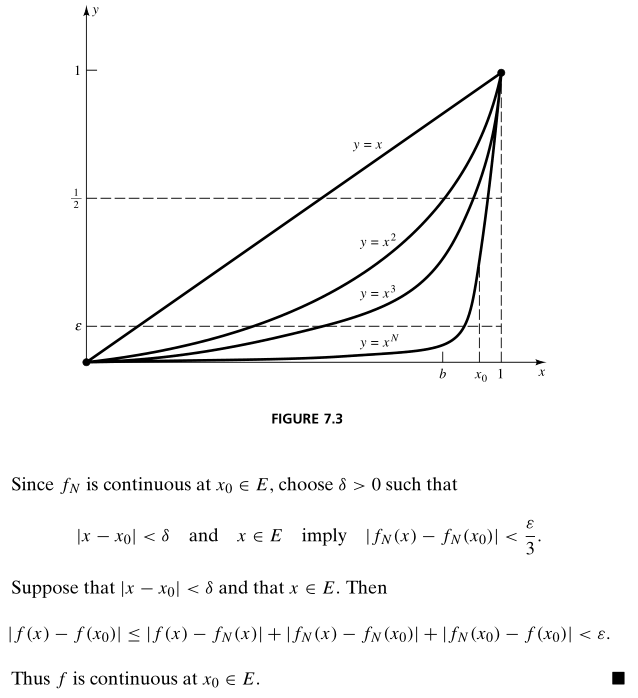
\includegraphics[width=250]{07_09b.png} \\
    07.10
    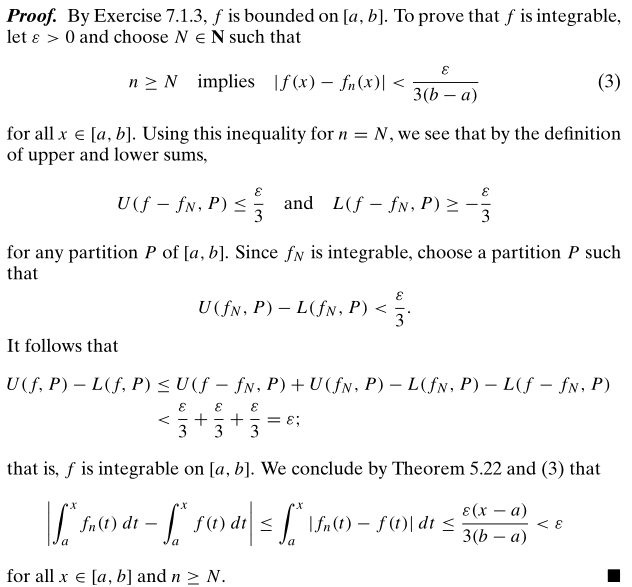
\includegraphics[width=250]{07_10.png} \\
    07.11
    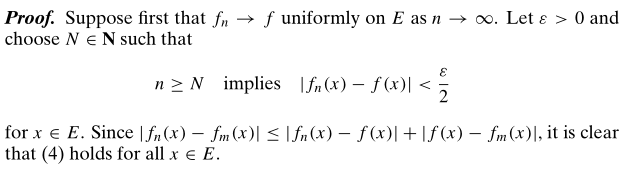
\includegraphics[width=250]{07_11a.png} \\
    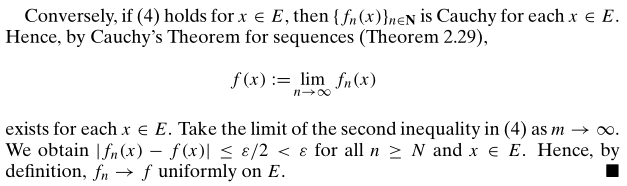
\includegraphics[width=250]{07_11b.png} \\
    07.12
    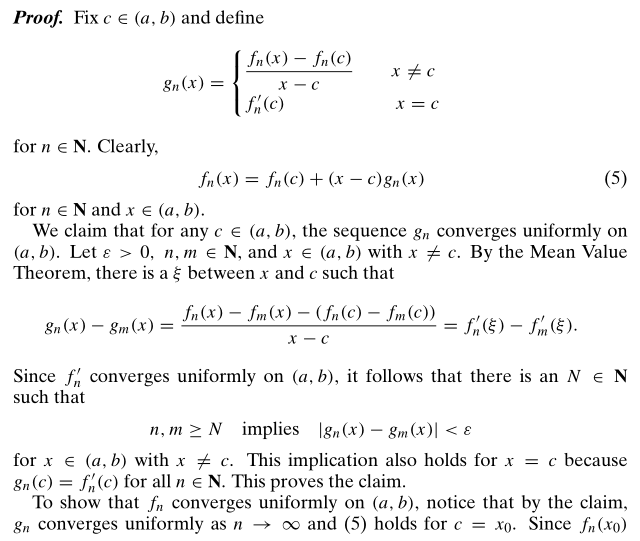
\includegraphics[width=250]{07_12a.png} \\
    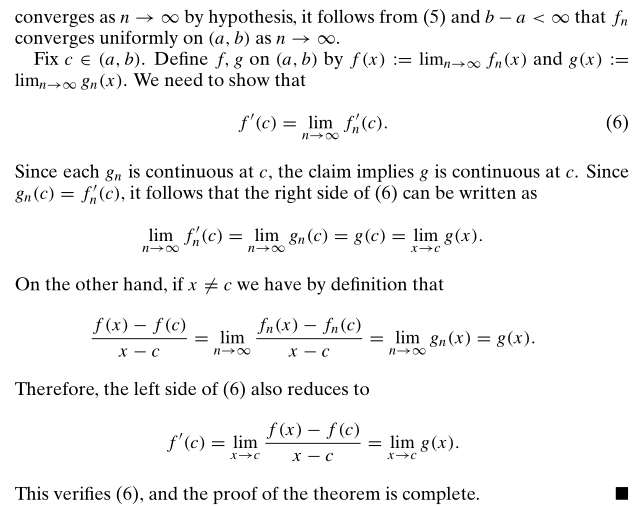
\includegraphics[width=250]{07_12b.png} \\
    07.15
    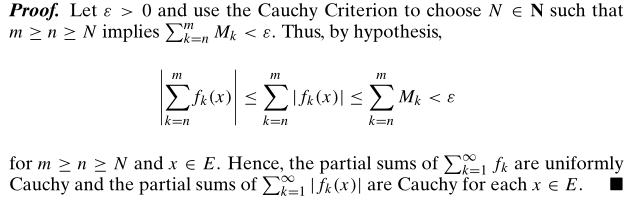
\includegraphics[width=250]{07_15.png} \\
    10.09
    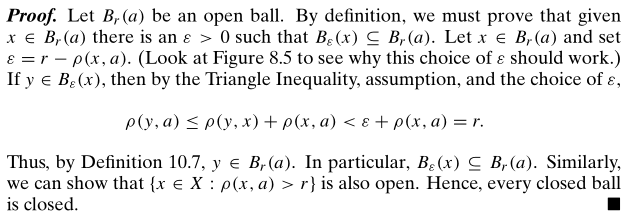
\includegraphics[width=250]{10_09.png} \\
    10.10
    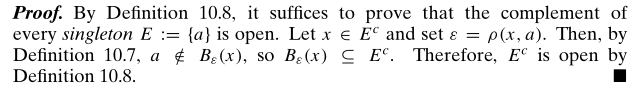
\includegraphics[width=250]{10_10.png} \\
    10.11
    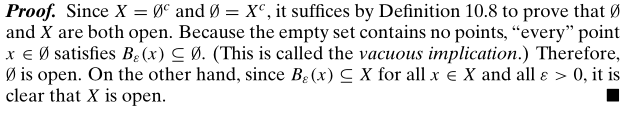
\includegraphics[width=250]{10_11.png} \\
    10.15
    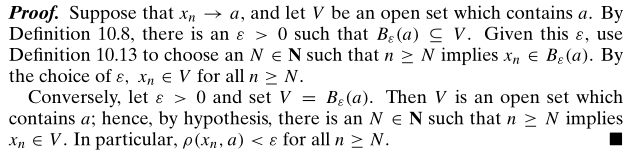
\includegraphics[width=250]{10_15.png} \\
    10.16
    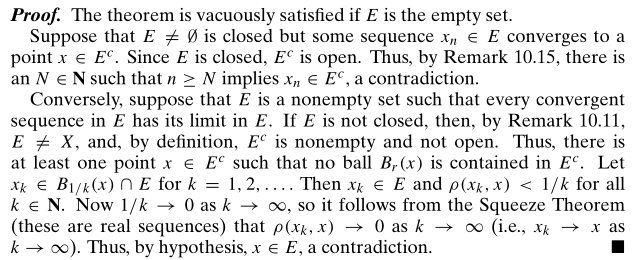
\includegraphics[width=250]{10_16.png} \\
    10.17
    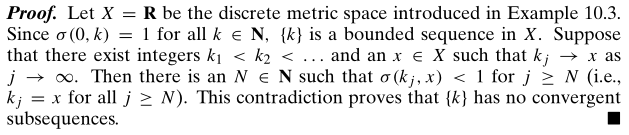
\includegraphics[width=250]{10_17.png} \\
    10.18
    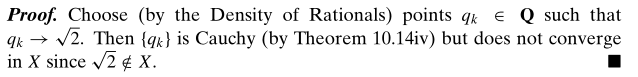
\includegraphics[width=250]{10_18.png} \\
    10.21
    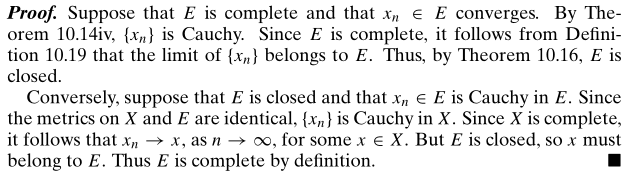
\includegraphics[width=250]{10_21.png} \\
    10.31
    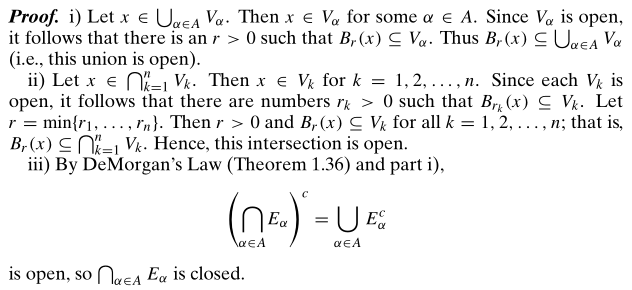
\includegraphics[width=250]{10_31a.png} \\
    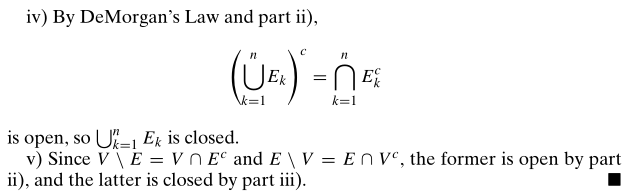
\includegraphics[width=250]{10_31b.png} \\
    10.32
    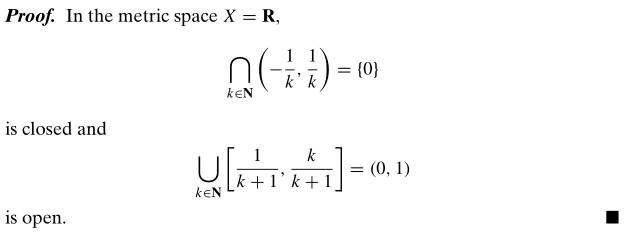
\includegraphics[width=250]{10_32.png} \\
    10.34
    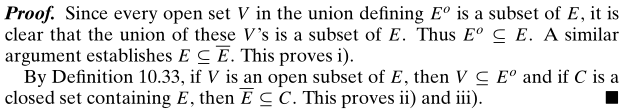
\includegraphics[width=250]{10_34.png} \\
    10.39
    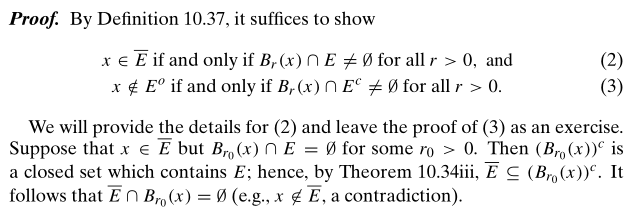
\includegraphics[width=250]{10_39a.png} \\
    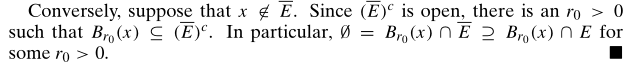
\includegraphics[width=250]{10_39b.png} \\
    10.40
    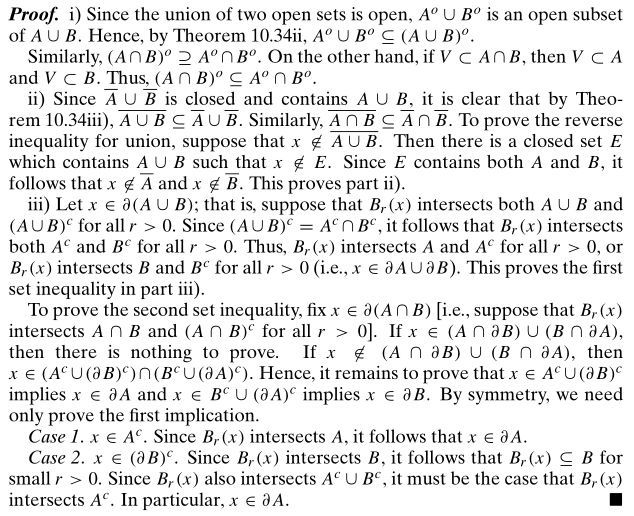
\includegraphics[width=250]{10_40.png} \\
    10.43
    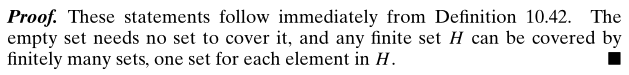
\includegraphics[width=250]{10_43.png} \\
    10.44
    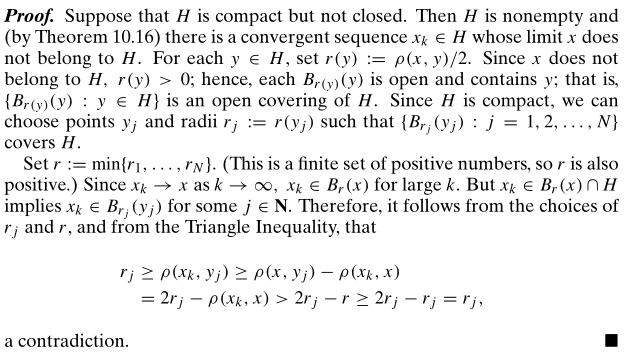
\includegraphics[width=250]{10_44.png} \\
    10.45
    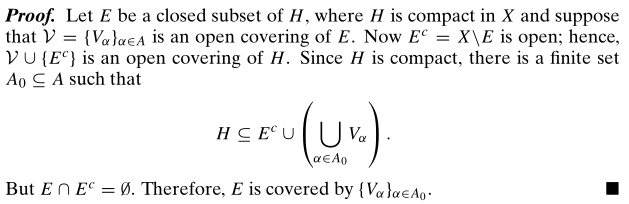
\includegraphics[width=250]{10_45.png} \\
    10.46
    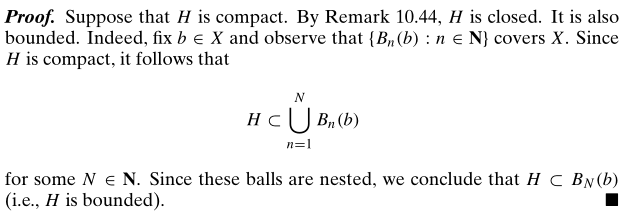
\includegraphics[width=250]{10_46.png} \\
    10.47
    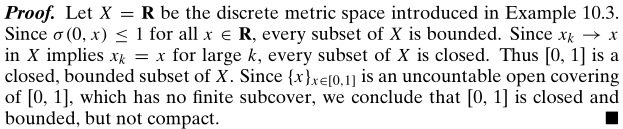
\includegraphics[width=250]{10_47.png} \\
    10.49
    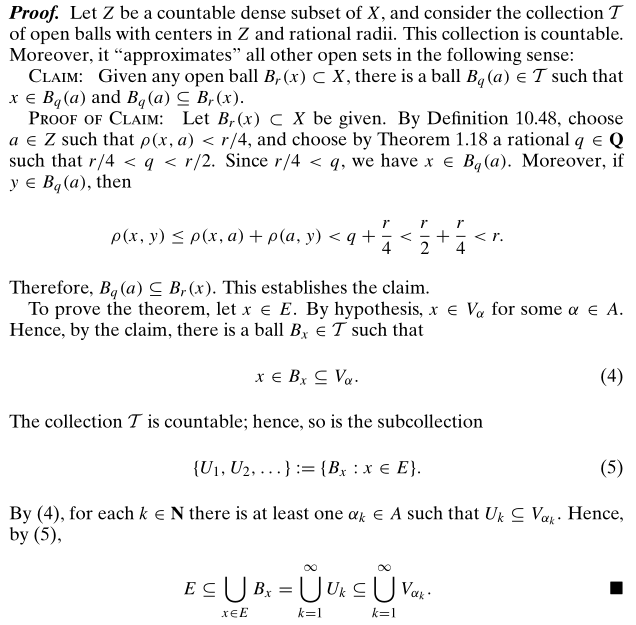
\includegraphics[width=250]{10_49.png} \\
    10.50
    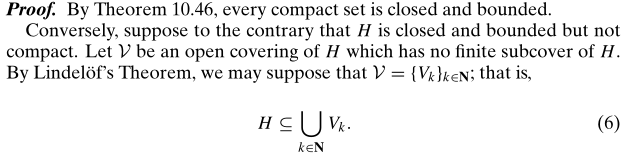
\includegraphics[width=250]{10_50a.png} \\
    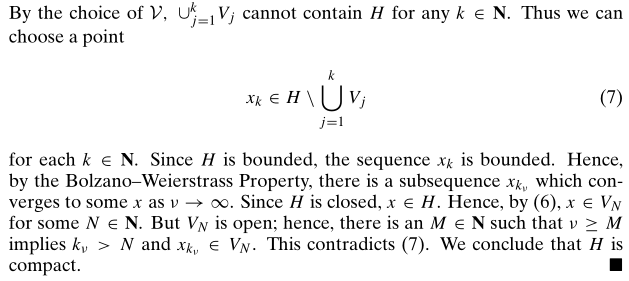
\includegraphics[width=250]{10_50b.png} \\
    10.52
    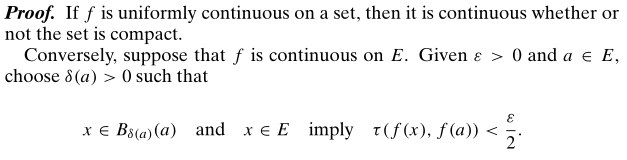
\includegraphics[width=250]{10_52a.png} \\
    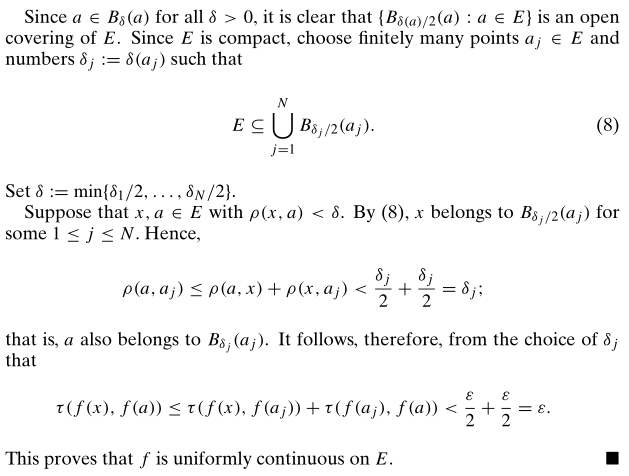
\includegraphics[width=250]{10_52b.png} \\
    10.55
    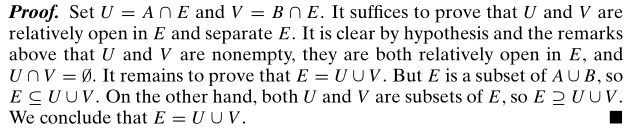
\includegraphics[width=250]{10_55.png} \\
    10.56
    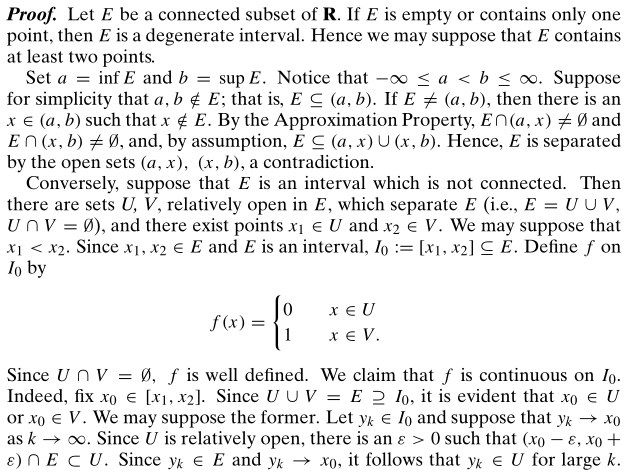
\includegraphics[width=250]{10_56a.png} \\
    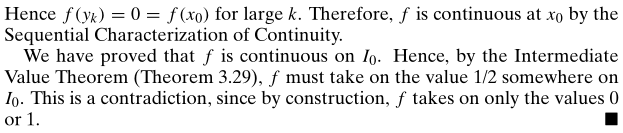
\includegraphics[width=250]{10_56b.png} \\
    10.58
    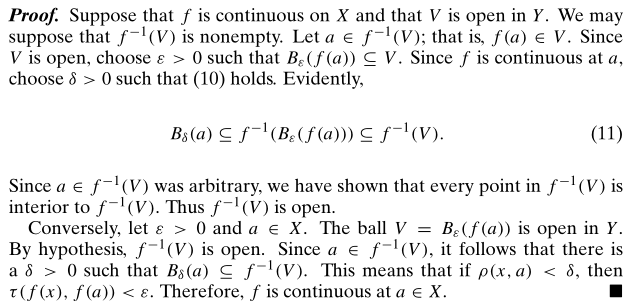
\includegraphics[width=250]{10_58.png} \\
    10.61
    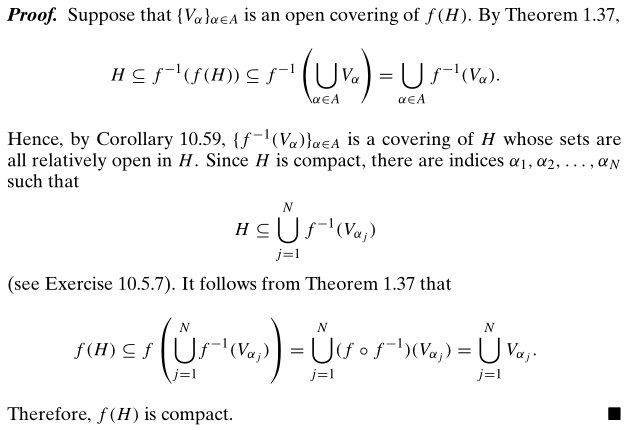
\includegraphics[width=250]{10_61.png} \\
    10.62
    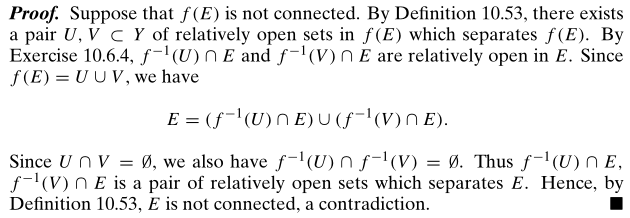
\includegraphics[width=250]{10_62.png} \\
    10.63
    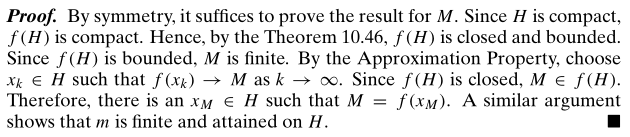
\includegraphics[width=250]{10_63.png} \\
    10.64
    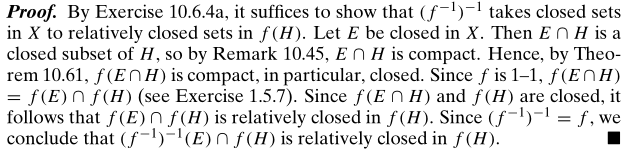
\includegraphics[width=250]{10_64.png} \\
\end{multicols}

\begin{multicols}{2}
    Riemann Prop 1
    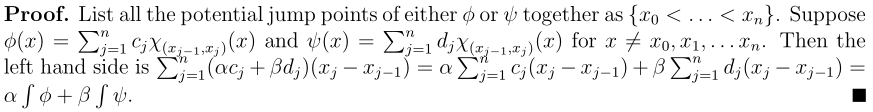
\includegraphics[width=400]{R_p1.png} \\
    Riemann Theorem 1
    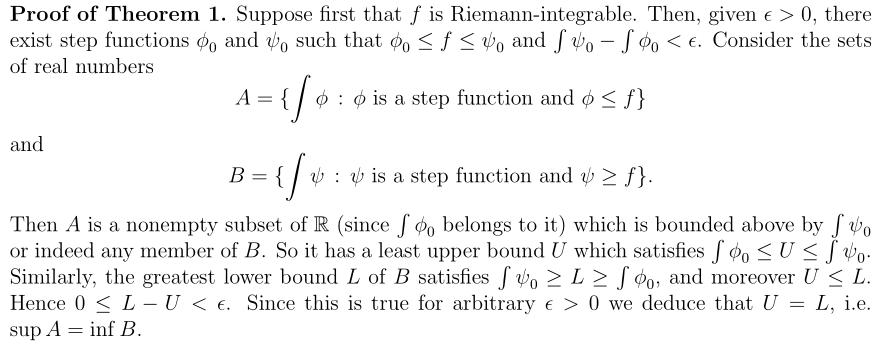
\includegraphics[width=400]{R_t1a.png} \\
    \includegraphics[width=400]{R_t1b.png} \\
    Riemann Theorem 1
    \includegraphics[width=400]{R_t2.png} \\
    Riemann Lemma 1
    \includegraphics[width=400]{R_l1a.png} \\
    \includegraphics[width=400]{R_l1b.png} \\
    Riemann Theorem 3
    \includegraphics[width=400]{R_t3.png} \\
    Riemann Theorem 4
    \includegraphics[width=400]{R_t4.png} \\
    Riemann Theorem 5
    \includegraphics[width=400]{R_t5.png} \\
    Riemann Theorem 6
    \includegraphics[width=400]{R_t6.png} \\
    Riemann Theorem 7
    \includegraphics[width=400]{R_t7a.png} \\
    \includegraphics[width=400]{R_t7b.png} \\

    Power Theorem 1
    \includegraphics[width=400]{P_t1.png} \\
    Power Theorem 2
    \includegraphics[width=400]{P_t2a.png} \\
    \includegraphics[width=400]{P_t2b.png} \\
    Power Lemma 1
    \includegraphics[width=400]{P_l1.png} \\
    Power Theorem 3
    \includegraphics[width=400]{P_t3.png} \\

    % \textbf{Contraction Mappings}
    Contraction Theorem 1
    \includegraphics[width=400]{B_t1a.png} \\
    \includegraphics[width=400]{B_t1b.png} \\
    % Contraction Theorem 2
    % \includegraphics[width=400]{B_t2a.png} \\
    % \includegraphics[width=400]{B_t2b.png} \\

\end{multicols}
\end{document}
